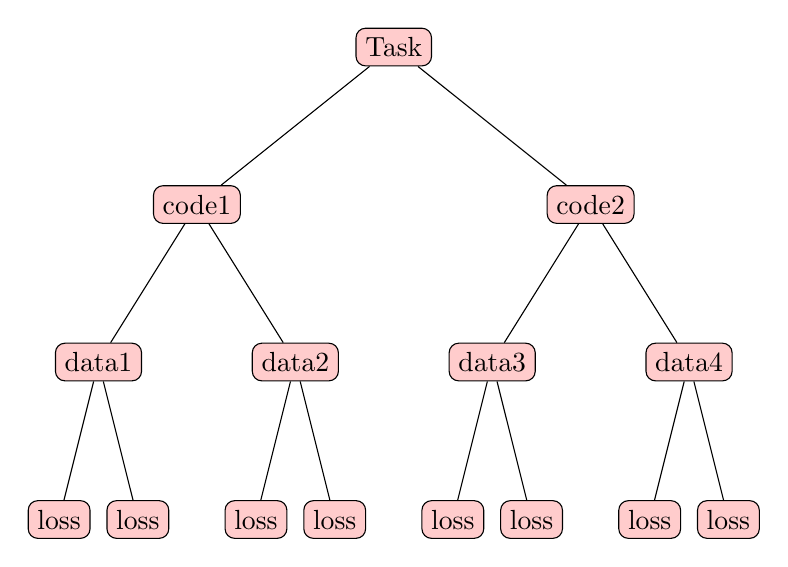
\begin{tikzpicture}
[
    level distance=2cm,
    level 1/.style={sibling distance=5cm},
    level 2/.style={sibling distance=2.5cm},
    level 3/.style={sibling distance=1cm},
    first/.style={level distance=6ex},
    second/.style={level distance=12ex},
    third/.style={level distance=18ex},
    common/.style={shape = rectangle, rounded corners=.8ex, draw, fill = red!20},
    highlight/.style={shape=rectangle, rounded corners=.8ex, draw, fill = red!50},
]
\node[common] {Task}
    child {node[common]{code1}
        child {node[common]{data1}
            child {node[common]{loss}}
            child {node[common]{loss}}
        }
        child {node[common]{data2}
            child {node[common]{loss}}
            child {node[common]{loss}}
        }
    }
    child {node[common]{code2}
        child {node[common]{data3}
            child {node[common]{loss}}
            child {node[common]{loss}}
        }
        child {node[common]{data4}
            child {node[common]{loss}}
            child {node[common]{loss}}
        }
    };
\end{tikzpicture}